\subsection{Self Training}
\label{sec:selftraining}

A database consists of $L$ speech waveforms, each containing $T$
frames with $M$ associated phone labels, $M<T$. 
The $\ell^{\textrm{th}}$ waveform is represented by acoustic feature
matrix $x^\ell =[x_1^\ell,\ldots,x_T^\ell]$, where $x_t^\ell$ is an
acoustic feature vector.  Its phone transcription
$\phi^\ell=[\phi_1^\ell,\ldots,\phi_M^\ell]$ determines the sequence
but not the durations of senones (HMM states) $s^\ell
=[s_1^\ell,\ldots,s_T^\ell]$.

The first set of PTs were computed using NN-HMM self-training.  The
Kaldi toolkit~\cite{Kaldi2011} was used to train a multilingual NN-HMM
in six languages not including the target language.  A training
script~\cite{vesely2013-semi} was then used to compute a senone
posterior probability $\rho(s_t^\ell|x_t^\ell)$ for each frame, and
the senone posteriors served as targets for re-estimating the neural
network weights.
%\begin{figure}
%  \centerline{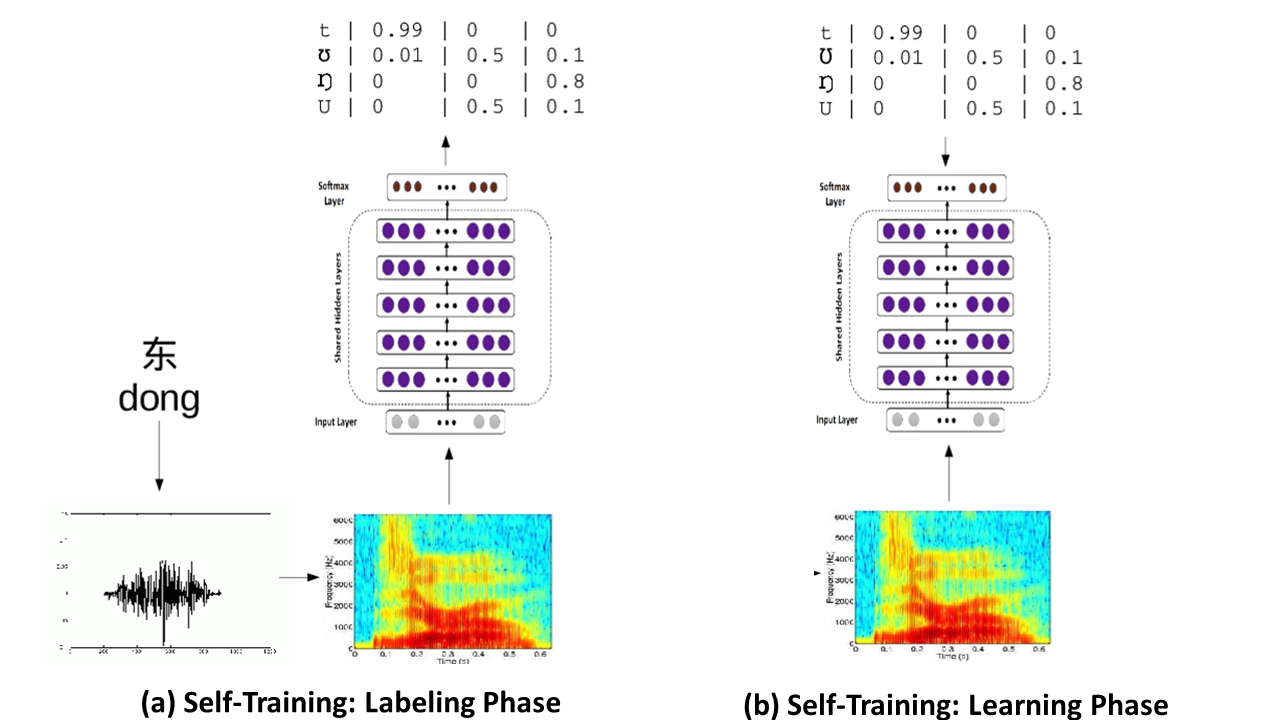
\includegraphics[width=5in]{../figs/fig_hager.png}}
%  \caption{The self-training method of~\cite{vesely2013-semi} includes
%    a labeling phase and a learning phase.  (a) Labeling phase: an ASR
%    trained on other languages (here Cantonese) is used to compute
%    posterior phone probabilities $\pi(\phi_t^\ell|x^\ell)$ in the
%    test language (here Mandarin). (b) Learning phase: posterior phone
%    probabilities are used as targets for NN re-training.}
%  \label{fig:hager}
%\end{figure}
%% comments: since the key difference in this figure between the
%% labeling phase and the learning phase is the direction of the upper
%% arrow, I suggest making the arrows more prominent. Also, the text
%% annotating the NN is illegible, as is the text garnishing the axes
%% of the waveform and spectrograms.
In contrast to the approach in \cite{vesely2013-semi}, which used the
best path alignment as the target in frame cross-entropy training, we
achieved better performance using the posteriors as soft-targets.
%(Fig.~\ref{fig:hager}). However, we did follow the recommendation in
%\cite{vesely2013-semi} to scale the amount of transcribed data by 2 to 
%create a good balance between transcribed and untranscribed data.
